\chapter{Overview}\label{s:overview}

\graphicspath{ {./images/} }
\begin{figure}[h]
\centering
\caption{a nice plot}
\label{fig:mesh1}
\end{figure}

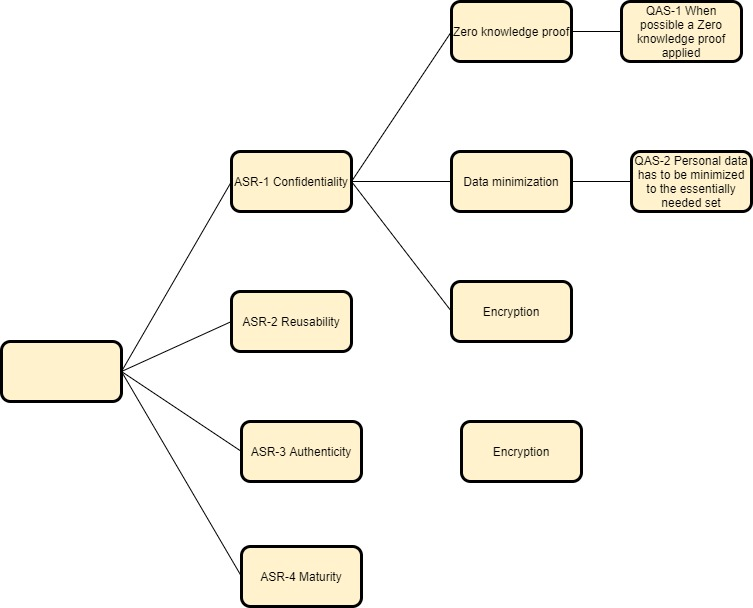
\includegraphics{universe.jpg}

There's a picture of a galaxy above

\begin{tabular}{ |p{5cm}||p{11cm}|}
 \hline
 \multicolumn{2}{|l|}{List of Business Goals} \\
 \hline
 BG-01 Explainable solutions   &   Communicate simple how technology works to raise awareness and support. Also, provide more detailed scientific information for experts to contribute as a community.     \\
 \hline
 BG-02 (Re-)Use of available standards and patterns &  Reusage of standards and patterns is a goal to keep systems maintainable and portable. It also helps in building a knowledge base that can be applied on multiple products \\
  \hline
 BG-03 Apply a 'Zero knowledge proof' or minimalize data exchange & "Minimalize the amount of data transfered. If data is not available it can not be stolen in case of for example a databreach.GDPR states a minimalization of data in Article 5. Only provide information that is needed for the initial purpose.
Ultimately, it's desired to only acknowledge if the provided personal information is correct, without providing the information itself. Also known as a 'Zero knowledge proof'."  \\
  \hline
BG-04 Maintain a unique identity of a person within a whole chain & Big advantage of maintaining a unique identity (number) of a person within a whole chain of government bodie, prevent rework and multiple different ways of administering a single person.  \\
  \hline
 BG-05 Provide ease of use and uniform (self)service solutions to a citizen, together with chain partners &  Services provided to citizens (both residential and non-residential) are uniformly provided by each government body. Currently, this is mainly provided by having a DigiD that is on itself based on the unique BSN of a citizen.\\
\end{tabular}

\begin{tabular}{ |p{3cm}||p{10cm}|}
 \hline
 \multicolumn{2}{|l|}{Business goal 1 - Explainable solutions} \\
 \hline
 Shorthand name   & BG-1 Explainable solutions    \\
 \hline
 Description &   Communicate simple how technology works to raise awareness and support. Also, provide more detailed scientific information for experts to contribute as a community.  \\
  \hline
 Stakeholders involved & Interviewee 3 - Directing architect  \\
  \hline
 Quality Requirements   & QA-xx, QA-xx, QA-xx, QA-xx \\
  \hline
 Concerns &   C-xx, C-xx, C-xx, C-xx, C-xx\\
  \hline
 Fitting this into Business Goal Scenario & AD \\
 \hline
\end{tabular}


\todo{
This section provides a high-level outline of the proposed system or solution.
It typically illustrates the system architecture or the interactions between the
different solution components (via a “boxes-and-arrows” diagram) from a user’s
perspective.
}